\subsection{Topological Configurations of the \(\chi\) Field: Solitons as Particles}
  \label{app:topological_solitons}

  \paragraph{Status of this construction.}
    The solitonic configurations described in this section are not introduced as
    fundamental degrees of freedom of Cosmochrony.
    They constitute \emph{effective geometric models} intended to illustrate how
    particle-like properties may emerge from stable configurations of the $\chi$
    field once a continuum and orientable geometric description becomes applicable.

    At the fundamental level, Cosmochrony does not assume a pre-existing spatial
    manifold, metric, or differential structure.
    A fully relational formulation, free of geometric presuppositions, is presented
    separately in Appendix~\ref{app:relational_formulation}.
    The present constructions should therefore be understood as phenomenological
    representations valid in the emergent geometric regime.

  In Cosmochrony, particles are interpreted as \textbf{topologically stable solitons} of the \(\chi\) field, where their
  properties---such as \textbf{spin, charge, and mass}---emerge from the \textbf{local deformation of \(\chi\)} and its
  topological structure.
  Below, we classify these configurations and explicitly link them to particle properties, emphasizing how
  \textbf{charge arises from the modulation of \(\chi\)'s relaxation}.

  \subsubsection{Charge as Local Deformation of \(\chi\)}
    The \textbf{sign of a particle's charge} (positive or negative) is determined by how it deforms the \(\chi\)
    field:
    \begin{itemize}
      \item A \textbf{positive charge} corresponds to a \textbf{local extension of \(\chi\)} (a "peak"), which resists relaxation and repels other positive charges (as two peaks cannot merge).
      \item A \textbf{negative charge} corresponds to a \textbf{local contraction of \(\chi\)} (a "trough"), which attracts positive charges (as a peak and trough can annihilate or merge).
    \end{itemize}
    This geometric interpretation explains \textbf{Coulomb-like interactions}
    without invoking a fundamental electromagnetic field, but as a consequence of \(\chi\) dynamics.

    \begin{figure}[h]
      \centering
      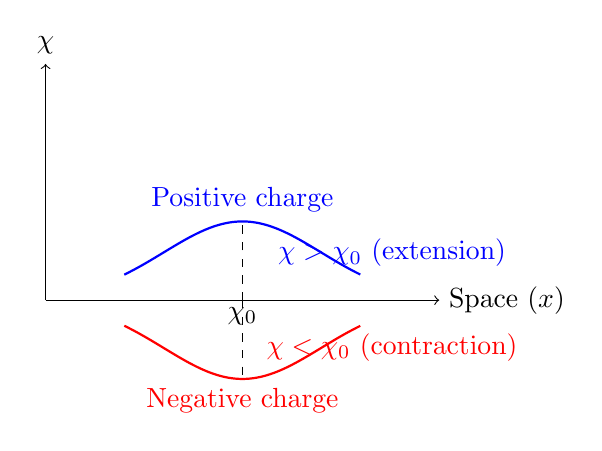
\begin{tikzpicture}[x=2cm, y=2cm]
        % Axes
        \draw[->] (0,0) -- (2.5,0) node[right] {Space (\(x\))};
        \draw[->] (0,0) -- (0,1.5) node[above] {$\chi$};
        % Positive charge: Peak in chi
        \draw[thick, blue, domain=0.5:2, samples=100] plot (\x, {0.5*exp(-2*(\x-1.25)^2)});
        \node[blue, above] at (1.25, 0.5) {Positive charge};
        \draw[dashed] (1.25,0) -- (1.25,0.5);
        \node at (1.25,-0.1) {$\chi_0$};
        % Negative charge: Trough in chi
        \draw[thick, red, domain=0.5:2, samples=100] plot (\x, {-0.5*exp(-2*(\x-1.25)^2)});
        \node[red, below] at (1.25, -0.5) {Negative charge};
        \draw[dashed] (1.25,0) -- (1.25,-0.5);
        % Labels
        \node[blue] at (2.2, 0.3) {$\chi > \chi_0$ (extension)};
        \node[red] at (2.2, -0.3) {$\chi < \chi_0$ (contraction)};
      \end{tikzpicture}
      \caption{
        Local deformations of the $\chi$ field representing positive (peak) and negative (trough) charges.
        The extension or contraction of $\chi$ relative to its background value $\chi_0$ determines the sign of the
        charge and the nature of its interactions (This figure and following ones are schematic representations intended
        to illustrate the geometric and topological structure of $chi$-field excitations, not numerical solutions of the
        dynamical equations.).
      }
      \label{fig:chi_charges}
    \end{figure}


  \subsubsection{Vortices (Charged Particles with Spin)}
    Vortices in the \(\chi\) field are characterized by a quantized winding number \(n\):
    \[
      n = \frac{1}{2\pi} \oint \nabla \arg(\chi) \cdot d\mathbf{l}.
    \]
    The \textbf{charge of the vortex} is determined by the \textbf{sign of its deformation}:
    \begin{itemize}
      \item For \(n > 0\), the vortex creates a \textbf{local extension of \(\chi\)} (positive charge).
      \item For \(n < 0\), the vortex creates a \textbf{local contraction of \(\chi\)} (negative charge).
    \end{itemize}
    The energy of the vortex scales with \(n^2\), reflecting the \textbf{mass of the particle}
    , while its winding determines the \textbf{spin} (e.g., \(n=1\) for spin-1 bosons).

    \begin{figure}[h]
      \centering
      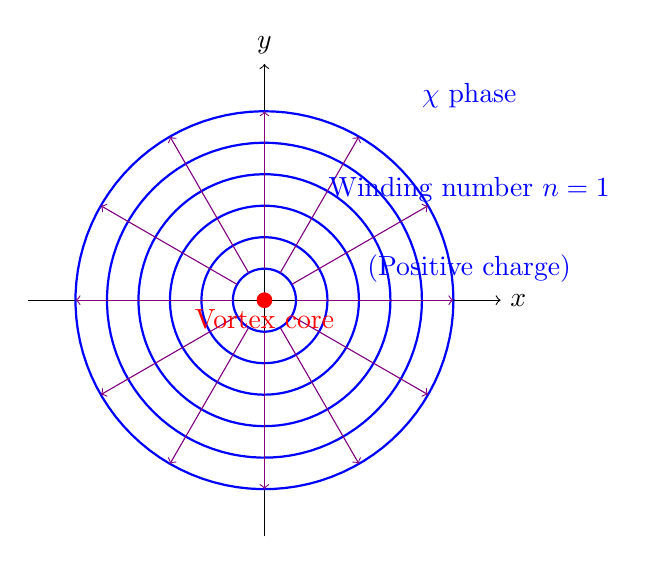
\begin{tikzpicture}[x=2cm, y=2cm]
        % Axes
        \draw[->] (-1.5,0) -- (1.5,0) node[right] {$x$};
        \draw[->] (0,-1.5) -- (0,1.5) node[above] {$y$};
        % Vortex field lines (streamlines of chi)
        \foreach \r in {0.2, 0.4, ..., 1.2} {
          \draw[blue, thick, domain=0:6.28, samples=100, variable=\t]
          plot ({\r*cos(\t r)}, {\r*sin(\t r)});
        }
        % Chi field phase (color gradient)
        \foreach \t in {0, 30, ..., 330} {
          \draw[red!50!blue, ->, domain=0.2:1.2, samples=20, variable=\r]
          plot ({\r*cos(\t)}, {\r*sin(\t)});
        }
        % Core of the vortex
        \fill[red] (0,0) circle (0.05);
        \node[red, below] at (0,0) {Vortex core};
        % Labels
        \node[blue] at (1.3, 1.3) {$\chi$ phase};
        \node[blue] at (1.3, 0.7) {Winding number $n=1$};
        \node[blue] at (1.3, 0.2) {(Positive charge)};
      \end{tikzpicture}
      \caption{
        Vortex configuration in the $\chi$ field, characterized by a winding number $n=1$.
        The circular phase gradient (arrows) represents the spin of the particle, while the core (red dot) corresponds to a localized deformation of $\chi$ (positive charge).
        Such configurations model charged bosons with quantized angular momentum.
      }
      \label{fig:chi_vortex}
    \end{figure}

  \subsubsection{Skyrmions (Fermions with Charge and Spin-1/2)}
    Skyrmions are 3D solitons with a topological charge \(Q\):
    \[
      Q = \frac{1}{4\pi} \int \mathbf{n} \cdot (\partial_x \mathbf{n} \times \partial_y \mathbf{n}) \, dx \, dy,
    \]
    where \(\mathbf{n} = \chi / |\chi|\).
    The \textbf{charge of the skyrmion} is linked to the
    \textbf{polarity of its \(\chi\) deformation}:
    \begin{itemize}
      \item A skyrmion with \(Q = +1\) and a \textbf{peak in \(\chi\)} represents a
      \textbf{positively charged fermion} (e.g., proton).
      \item A skyrmion with \(Q = -1\) and a \textbf{trough in \(\chi\)} represents a
      \textbf{negatively charged fermion} (e.g., electron).
    \end{itemize}
    The \(4\pi\)-periodicity of skyrmions under rotations explains their \textbf{spin-1/2}
    nature, while the deformation of \(\chi\) accounts for their charge.

    \begin{figure}[h]
      \centering
      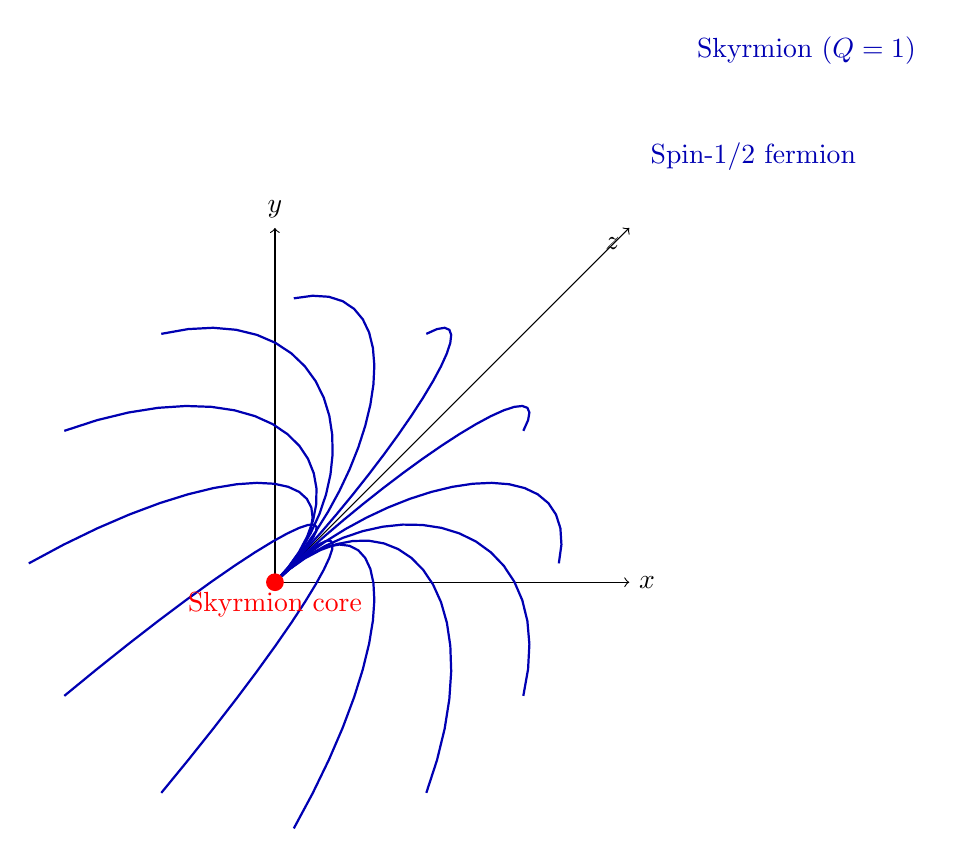
\begin{tikzpicture}[x=1.5cm, y=1.5cm, z=1.5cm, scale=1.5]
        % Axes
        \draw[->] (0,0,0) -- (2,0,0) node[right] {$x$};
        \draw[->] (0,0,0) -- (0,2,0) node[above] {$y$};
        \draw[->] (0,0,0) -- (0,0,2) node[below left] {$z$};
        % Skyrmion field (simplified representation)
        \foreach \phi in {0, 30, ..., 330} {
          \draw[blue!70!black, thick, domain=0:1.5, samples=20, variable=\r]
          plot ({\r*sin(deg(\r))*cos(\phi)}, {\r*sin(deg(\r))*sin(\phi)}, {\r*cos(deg(\r))});
        }
        % Core and labels
        \fill[red] (0,0,0) circle (0.05);
        \node[red, below] at (0,0,0) {Skyrmion core};
        \node[blue!70!black] at (1.5, 1.5, 1.5) {Skyrmion ($Q=1$)};
        \node[blue!70!black] at (1.5, 1.2, 1.2) {Spin-1/2 fermion};
      \end{tikzpicture}
      \caption{
        Skyrmion configuration in the $\chi$ field, with topological charge $Q=1$.
        The 3D structure reflects the fermionic nature of the particle (spin-1/2), where the core (red dot) represents a localized excitation of $\chi$.
        Skyrmions provide a geometric model for fermions, with their charge determined by the polarity of the $\chi$ deformation.
      }
      \label{fig:chi_skyrmion}
    \end{figure}

  \subsubsection{Summary: Topology and Charge}
    The relationship between topology and charge in Cosmochrony is summarized in ~\ref{tab:solitons_charge}

    \begin{table}[htbp]
      \centering
      \caption{Topological Solitons, Charge, and \(\chi\) Deformation}
      \label{tab:solitons_charge}
      \begin{tabular}{|c|c|c|c|}
        \hline
        \textbf{Soliton Type} & \textbf{Topological Invariant} & \textbf{\(\chi\) Deformation} &
        \textbf{Particle Property} \\
        \hline
        Vortex & Winding number \(n\) & Peak (\(n>0\)) or trough (\(n<0\)) & Charge
        \(\propto n\), spin \(\propto |n|\) \\
        Skyrmion & Charge \(Q\) & Peak (\(Q>0\)) or trough (\(Q<0\)) & Charge
        \(\propto Q\), spin-1/2 \\
        \hline
      \end{tabular}
    \end{table}
